\documentclass[a4paper,11pt]{article}
\usepackage{amsmath}
\usepackage{amsfonts}
\usepackage{titling}
\usepackage{graphicx}
\usepackage[utf8]{inputenc}
%\newcommand{\location}[1]{}
%\newcommand{\publication}[1]{}
\newcommand{\textbb}[1]{\textbf{#1}}
\newcommand{\WTF}[1]{\textbf{???}\textit{#1}\textbf{???}}
\newcommand{\?}[2]{#1\footnote{\textsc{Translator note}: #2}}
\newcommand{\nequ}[2]{\begin{align*}\tag{#1}#2\end{align*}}
\newcommand{\uequ}[1]{\begin{align*}#1\end{align*}}
\newcommand{\unit}[1]{\text{#1}}
\providecommand{\operatorfont}[1]{\texttt{#1}}
%\newcommand{\operatorfont}[1]{}
\newcommand{\grad}{\operatorfont{grad}}
\renewcommand{\div}{\operatorfont{div}}
\newcommand{\curl}{\operatorfont{curl}}
\newcommand{\rot}{\,\operatorfont{rot}\,}
\renewcommand{\exp}[1]{e^{#1}}
\newcommand{\pXpY}[2]{\frac{\partial #1}{\partial #2}}
\newcommand{\ppXpYY}[2]{\frac{\partial^2 #1}{\partial {#2}^2}}
\newcommand{\dXdY}[2]{\frac{d{#1}}{{d{#2}}}}
\newcommand{\ddXdYY}[2]{\frac{d^2{#1}}{d{#2}^2}}
\newcommand{\mf}[1]{\mathfrak{#1}}
\newcommand{\Nth}[1]{{#1}^\text{th}}

\newcommand{\citeauthor}[1]{\textsc{#1}}
\newcommand{\citetitle}[1]{\textit{#1}}
\newcommand{\citepub}[1]{#1}
\newcommand{\citevol}[1]{\textbf{#1}}
\newcommand{\citepage}[1]{#1}
\newcommand{\citedate}[1]{#1}
\newcommand{\citeyear}[1]{#1}

\newcommand{\El}[1]{\text{#1}}
\newcommand{\mnEl}[3]{{}^{#1}_{#2}{\El{#3}}}

\newcommand{\publication}[1]{%
    \gdef\puB{#1}}
\newcommand{\puB}{}
\renewcommand{\maketitlehooka}{%
    \par\noindent \puB}


\newcommand{\location}[1]{%
    \gdef\loB{#1}}
\newcommand{\loB}{}
\renewcommand{\maketitlehooka}{%
    \par\noindent \loB}

%\newcommand{\dX}[2]{\frac{d#1}{{#2}}}
%\newcommand{\dY}[1]{{d#1}}
%\newcommand{\pX}[1]{\frac{\partial{#1}}}
%\newcommand{\pY}[1]{{\partial{#1}}}

% \newcommand{\original}[1]{}
\newenvironment{translation}[0]{
}

\newenvironment{original}{
\renewcommand{\footnote}[1]{\small{(Footnote: ##1)}}
(\textit{Begin original text}:
}{
\textit{-- end original text})
}


\begin{document}

\title{General theoretical considerations on the structure of nuclei}

\author{Werner Heisenberg}
\location{Solvay}
\publication{Solvay 1933}
\date{fixme}

\maketitle

\tableofcontents

\section{Review of principles.}

Since the experimental data concerning the structure of the atomic nucleus has not up to now brought us any new physical notions going beyond quantum mechanics, it is necessary to examine at the start of a theoretical \?{expositiontion}{expos\'e} on the nucleus to what extent the quantum or wave mechanics may be utilized in this new domain. Narrowing down as much as possible the scope of applicability of wave mechanics is one of the first tasks in the theory of the nucleus.

Gamow, Condon and Gurney\footnote{\citeauthor{G. Gamow}, \citetitle{Der Bau des Atomkerns und die Radioaktivit\"at} (Leipzig, 1932).} have shown in their theory on $\alpha$ decay that the heavy constituents of the nucleus ($\alpha$ particles and protons) are subject to energetic conditions on the inside analogous to those affecting the electrons in the atom outside of the nucleus. The decay energies of the radioactive elements and those which are necessary for the decay of light nuclei are small with respect to the \?{self-energy}{\'energie propre} of the heavy corpuscules (if $M$ is the mass of the proton, $c$ the speed of light, one has $Mc^2 = 1.5\cdot 10^{-3}\unit{erg}$; the decay energies are between $10^{-6}$ and $10^{-5}\unit{erg}$). Correspondingly, the measured nuclear radii are notably larger than the characteristic length of the relativistic effects of protons, $\frac{\hbar}{Mc} = 2\cdot 10^{-14}\unit{cm}$. One may as a consequence expect that quantum mechanics, in its current form, would be applicable to the motion of heavy particles in the atomic nucleus and that the fundamental notions introduced by Bohr in the theory of quanta (stationary states, frequency relations, transition probability) can be extended to these particles, and finally that the developments of quantum mechanics in the direction of the theory of relativity only play a secondary role here.

In fact, the existence of discontinuous series of decay energies, their connection with the lines of the $\gamma$ spectrum, and the success of the theory of $\alpha$ decay (\textit{see} Gamow's report) show that the heavy nuclear constituents behave in a manner consistent with quantum mechanics.

Bohr\footnote{\citeauthor{N. Bohr}, \citetitle{Atomic stability and conservation laws}, \citepub{Convegno di Fisica nucleare} (Rome 1932).} has indicated a simple qualitative relation between the size of the nuclei and their mass defects, as a consequence of the applicability of quantum mechanics to the motion of heavy particles inside the nucleus. If, for example, $r_a$ represents the position of a helium nucleus, the following expression for the domain of variation $\Delta p$ of the momentum of a proton in the interior of a helium nucleus results from the uncertainty relations:
\nequ{1}{
\Delta p \approx \frac{\hbar}{r_0}
}
and hence for its mean kinetic energy
\nequ{2}{
\overline{E}_\text{kin} \approx \frac{1}{2M}\left(\frac{\hbar}{r_0}\right)^2.
}

Like in general the mean kinetic energy of a particle is of the same order of magnitude as the mean potential energy and as the total energy, one obtains for the mass defect of the helium nucleus, measured in energy, a value of the order $4\cdot\frac{1}{2M}\left(\frac{\hbar}{r_0}\right)^2$. If, following Chadwick's experiments, we assume
\uequ{
r_0 \approx \frac{e^2}{mc^2} = 2.8\cdot 10^{-13}\unit{cm}
}
($m$ the mass of the electron), then
\uequ{
\text{mass defect} \approx 4\times\frac{1}{2M}(mc)^2\left(\frac{\hbar c}{e^2}\right)^2 \approx 0.01 Mc^2,
}
of the same order of magnitude as the experimental value $0.029Mc^2$.

These considerations call for two remarks which will be used for the later discussion: in the first place we have completely ignored the contribution to the mass defect of negative charges which may be contained in the nucleus, and this may not be justified from the point of view of quantum mechanics; in the second place, it must be highlighted that the forces ensuring the cohesion of the nucleus are certainly of a different nature than Coulomb's, which are introduced in the application of quantum mechanics on external electrons. In fact the Coulomb forces would give in the helium nucleus a mass defect of order
\uequ{
\frac{(2e)^2}{r_0}\approx 4mc^2 = 0.002Mc^2,
}
that is to say only a fifteenth of the experimental mass defect. From this we deduce that, in light atoms, the Coulomb forces only have a secondary importance with respect to other unknown actions, and that they only become important in heavy nuclei, since they increase as the square of the nuclear charge. We do not yet have any theoretical means for studying the forces which act in the nucleus between the various heavy constituents; however the current experimental data permit drawing some general conclusions on the nature of these forces. We later examine this point in more detail.

If one is to interpret the fact that certain atomic nuclei decay with the emission of $\beta$ rays by assuming that the negative electrons appear in the same way as the $\alpha$ particles and the protons, as independent constituents of the nucleus, one is immediately struck by a group of difficulties of principle whose solution does not seem to be possible in the current state of the theory. It is known that quantum mechanics treats electrons as point charges which act on one another in accordance with the laws of the Maxwell theory. This manner of proceeding however is only admissible of the distances between the point charges are large with respect to $\frac{e^2}{mc^2}$. In fact, the theory of the inertia of energy permits confirming that the Coulomb law ceases being exact at distances to the center of the electron on an order smaller than $\frac{e^2}{mc^2}$, $m$ being the mass of the electron. This result may again be expressed by saying that the distance of the electron is on the order of $\frac{e^2}{mc^2}$. On the other hand, since the linear dimensions of the atomic nucleus are not much larger than $\frac{e^2}{mc^2}$, there can be no question of applying quantum mechanics to the motion of electrons inside the nucleus. Thus the circumstsnces in which nuclear electrons are found are so distant from the domain of applicability of the known laws that no conclusion concerning the motion of the light constituents in the atomic nucleus can be obtained, neither by Lorentz's electron theory, nor by quantum mechanics, nor even by application of the correspondence principle. It also means, as a final consequence, that the assertion "the electrons appear as nuclear constituents" has no definite meaning, despite the fact related earlier that many nuclei emit $\beta$-rays. 

To this situation corresponds the experimental fact that anywhere the behavior of negative charges in the interior of the nucleus is involved, experiment leads to results without analogy to the laws known today. For example, while quantum mechanics predicts the validity of Bose statistics for systems constituted of protons and electrons of even total \textit{charge} and integer angular momentum, and Fermi statistics when the total \textit{charge} is odd and the angular momentum is an odd multiple of $\frac{1}{2}$, it seems that the statistics and the angular momentum of a given nucleus are in reality dependent on the parity of its \textit{mass}\footnote{C.f. \citeauthor{S. Goudsmit}, \citepub{Phys. Rev.}, \citevol{43}, \citeyear{1933}, \citepage{p. 636}, and \citeauthor{E. Fermi and E. Segré}, \citepub{Zeits. f. Phys.} \citevol{82}, \citeyear{1933}, \citepage{p. 729}.}

In addition, while the energy of a particle lost during a decay must be entirely defined by the difference in mass of the nucleus before and after the decay, it seems that no relation that simple is satisfied in the case of the emission of primary $\beta$-rays\footnote{Cf. \citeauthor{Bohr}, \citepub{Convegno di Fisica nucleare} (Rome, \citeyear{1932})}.

Beyond this difficulty resulting from direct experience, there are others when attempting to develop a theoretical test of the behavior of nuclear electrons with the aid of quantum mechanics. First of all, it seems impossible from the point of view of Dirac's theory of the electron that an electron should lie in the vicinity of order $\frac{e^2}{mc^2}$ of a proton (\textit{cf.} the Klein paradox). Otherwise, an application of the uncertainty relations to the motion of an electron in the nucleus leads, by analogy with the equations (1) and (2), to momenta on the order of 
\nequ{3}{
\Delta p \approx \frac{\hbar}{r_0} = \frac{\hbar c}{e^2}mc,
}
and to a mean kinetic energy
\nequ{4}{
\overline{E}_\text{kin} \approx \Delta p\times c \approx 
\frac{\hbar c}{e^2}mc^2 \approx 137 mc^2.
}

If we want to conclude that, as with the proton, the mass defect must be of the same order of magnitude as the mean kinetic energy, one obtains values for the mass defect that are much too large because of the presence of an electron in the nucleus. But, Bechert\footnote{I am indebted to M. Bechert for his communication by letter of the reasoning which follows.} has shown that even in the Coulomb field, it is not legitimate to evaluate the total energy $\mathcal{E}$ from the kinetic energy. From the equation
\nequ{5}{
\overline{\sum\limits_k(\dot{p}_k q_k + p_k\dot{q}_k)} = 
\overline{\sum\limits_k\dXdY{}{t}(p_k q_k)} = 0
}
gives in the case of the Coulomb field
\uequ{
+\overline{E}_\text{pot} + \overline{\sum\limits_k\frac{m_k \dot{q}_k^2}{\sqrt{1-\beta_k^2}}} = \overline{E}_\text{pot} + \overline{E}_\text{kin}
+\overline{\sum\limits_s\left(m_s c^2 - m_s c^2 \sqrt{1-\beta_s^2}\right)} = 0
}
and consequently
\nequ{6}{
\mathcal{E} = -\overline{\sum m_s c^2 - \left(1- \sqrt{1-\beta_s^2}\right)}.
}

The mass defect per electron is then always less than $mc^2$ in the case of the Coulomb field. It is of course impossible to say if this result is applicable to the theory of the nucleus since, as seen earlier, actions inside the nucleus certainly do not follow the Coulomb law.

The claim that the laws of quantum mechanics may be applied only to the heavy constituents of the nucleus, to the exclusion of the electrons, \?{is not to be accepted without reservation, due to the fact that}{comporte quelque réserve du fait que}, according to the quantum theory itself the protons may not be the only constituents of the nucleus, since they are repelled according to the Coulomb law, and it is thanks to the presence of negative charges that the \?{clustering}{association} of protons in the nucleus is rendered possible. In any case, a clear separation of the domains in which quantum mechanics is or is not applicable may only be obtained with a clearly-defined hypothesis concerning the structure of the atomic nucleus.


\section{Hypotheses on the structure of nuclei.}

When seeking to represent the structure of the atomic nucleus in more detail, one must first of all take into account the essential fact that the masses of the nuclei are evidently integer multiples of a quarter of the atomic mass of helium, and not integer multiples of the proton mass. It seems as a result that the atomic nuclei are formed in large part by $\alpha$ particles, which is confirmed by the fact that radioactive nuclei can decay with the emission of $\alpha$-rays. To the question of knowing the other constituents of the nucleus, one may respond in various ways, among which \?{experiment does not yet permit a decisive choice}{l'expérience ne permet pas encore de trancher de manière décisive}.

\subsection{Gamow's "drop" model.}

Gamow has assumed that $\alpha$ particles, which act on one another with forces that decrease very rapidly as a function of distance, may \?{be brought back together with}{s'associer encore des} negative charges (nuclear electrons); \?{besides these electrons}{en dehors de ces electrons}, free protons may still exist in the nucleus. The actions between $\alpha$ particles are envisaged by Gamow as analogous to the Van der Waals forces between molecules; thus he assumes first of all a finite distance for the $\alpha$ particle, with a rapidly-decreasing attractive action that is replaced by the Coulomb repulsion as the distance increases. The atomic nucleus thus appears as a system which may be compared to a liquid droplet whose cohesion is the result of the action of surface tension. This idea of Gamow's gives a good account of the experimental fact that the mean density of the nucleus seems to be nearly independent of its dimensions (the nuclear radius increases as the cubic root of the atomic mass). In addition, it allows predicting, at least qualitatively, the observed diminution of the mass defect per $\alpha$ particle when the atomic mass increases and attributes it to the influence of the Coulomb forces. On the contrary, the hypothesis of the nuclear electrons leads to these difficulties: the Coulomb forces on these electrons cannot account for the value of the mass defect per nuclear electron, the experimental value appearing too large. Further, the experimental result indicated earlier concerning the spin and statistics of the nucleus oblige us to assume that nuclear electrons have an integer angular momentum and follow Bose statistics, in contradiction with the accustomed properties of the electron. Finally, it is difficult to understand why, despite the mutual energetic action between the electrons and the $\alpha$ particles, the decay energies for $\alpha$ emission have well-defined values, while the primary $\beta$-ray spectrum is virtually continuous.

Gamow's "drop" model leads to attributing to a nucleus composed solely of $\alpha$ particles an energy of the form
\nequ{7}{
\mathcal{E} = C.N_\alpha + \frac{(2eN_\alpha)^2}{r},
}
where $N_\alpha$ represents the number of $\alpha$ particles and $r$ the radius of the nucleus. The first term on the left corresponds to rapidly-decreasing attractive forces between the $\alpha$ particles, and the second to the Coulomb forces. Writing:
\uequ{
r=R\sqrt[3]{N_\alpha},
}
one gets
\nequ{8}{
\mathcal{E} = -CN_\alpha + 4\frac{e^2}{R}(N_\alpha)^\frac{5}{3}.
}

The mass defect curve represented by equation (8) has a minimum and predicts that nuclei containing a large number of $\alpha$ particles must decay spontaneously with $\alpha$ emission. For nuclei containing electrons as well as $\alpha$ particles, Gamow posits equations analogous to (8), but which cannot be deduced directly from the model. From the hypothesis that the stability of a nucleus with respect to $\beta$ decay may be determined by the energy balance of the decay processes under consideration, and utilizing the mass defects observed by Aston, Gamow obtains the known pattern of figure 1 for the mass defect as a function of the number of electrons and $\alpha$ particles. We return later to the legitimacy of the hypothesis concerning the stability with respect to $\beta$ decay.

\begin{figure}[h!]
\centering
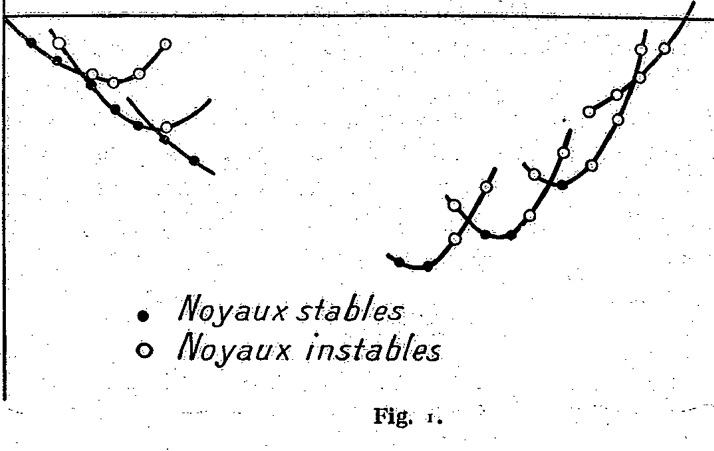
\includegraphics[width=200pt]{images/figure1}
\end{figure}

The numerous difficulties which lead, as will be seen, to the introduction of nuclear electrons make it necessary for us to examine as well the other possible hypotheses for the structure of the nucleus.

\subsection{Introduction of neutrons as nuclear constituents.}

First, on the new possibilities resulting from the discovery of the neutron by Curie and Joliot\footnote{\citeauthor{I. Curie \& F. Joliot}, \citepub{C.R. Acad. Sc.} \citevol{194}, \citeyear{1932}, \citepage{p.273, 876.}} and by Chadwick\footnote{\citeauthor{J. Chadwick}, \citepub{Nature}, \citeyear{1932}, \citepage{312}; \citepub{Proc. Roy. Soc.}, \citevol{17136}, \citeyear{1932}, \citepage{692}.}. This discovery does not only concern the existence of a corpuscule of mass 1 and charge 0, but shows in a certain manner who these neutrons may figure as independent constituents of the nucleus alongside the protons  and $\alpha$-particles. The experimental laws relative to spin and statistics of nuclei lead to the assumption that the neutron follows Fermi statistics and its spin is an odd multiple of $\frac{1}{2}$. This leads to assuming the value $\frac{1}{2}$ for the neutron's spin.

Several arrangements for the structure of the nucleus are compatible with this and are obtained by introducing as nuclear constituents alongside the $\alpha$ particles the neutrons, the protons and the electrons, or only the neutrons and the protons. These arrangements have been discussed very completely by Perrin\footnote{\citeauthor{F. Perrin}, \citepub{Soc. Franc.}, \citevol{324}, \citeyear{1932}, \citepage{96}; \citepub{C.R. Acad. Sc.}, \citevol{194}, \citeyear{1932}, \citepage{343}; \citevol{194}, \citeyear{1932}, \citepage{2211}; \citevol{195}, \citeyear{1932}, \citepage{236}.}, Iwanenko\footnote{\citeauthor{D. Iwanenko}, \citepub{Nature}, \citevol{129}, \citeyear{1932}, \citepage{312}.}, Gapon\footnote{TODO}, Bartlett\footnote{TODO}, and Land\'e\footnote{TODO}; it will suffice in this report to show on some atomic nuclei chosen as examples the characteristic differences of these various arrangements. (Here we employ the nuclear symbols $\El{He} = \mnEl{4}{2}{He}$, proton = $\mnEl{1}{1}{H}$, neutron $\mnEl{1}{0}{n}$, electron = $\varepsilon^-$.)

\begin{figure}[h!]
\centering
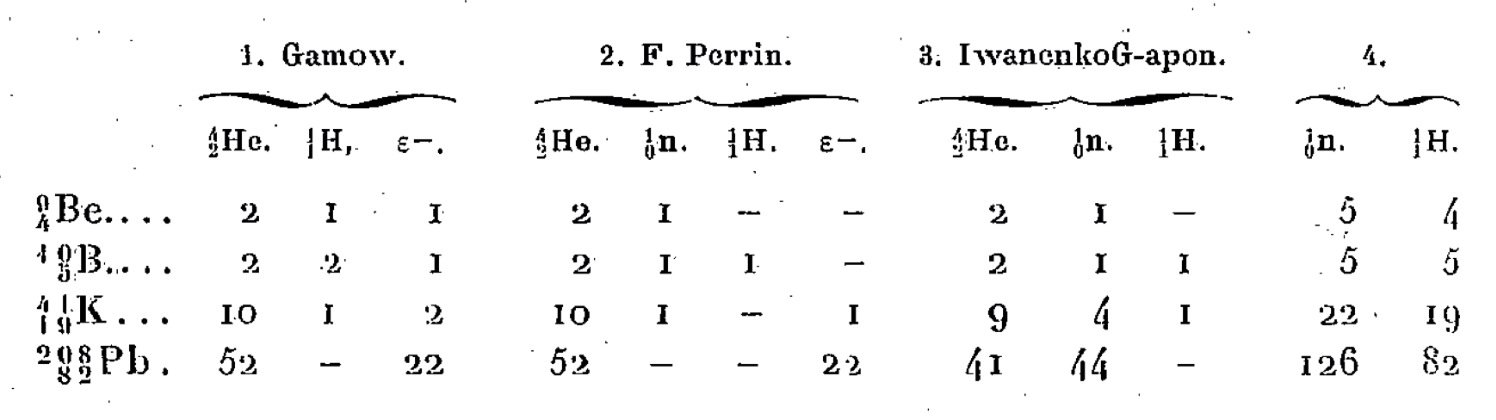
\includegraphics[width=350pt]{images/table1}
\end{figure}

The last column contains a different expression from that contained in the preceding; there one also considers the $\alpha$ particles as composed of two neutrons and two protons. The arrangement in column 2 considers the neutrons as elementary constituents that are non-dissociable and, to account for the $beta$ decay of radioactive elements, introduces explicitly, alongside the neutrons, electrons as constituents of the nucleus. Although this conception leads to interesting points of view on the $\beta$ radioactivity of the elements — F. Perrin related for example the $\beta$ activity of $\El{K}_{41}$ to the first appearance of a nuclear electron (cf table I) — it raises the same objections as Gamow's arrangement I because of the introduction of free nuclear electrons. On the other hand, conceptions .[3 and 4 interpret the empirical laws concerning the spin and statistics  of the nuclei by making an appeal to the \WTF{simple properties} of the {neutron, but they run up against difficulties with $\beta$ activity; in {fact, it must be admitted in conceptions 3 and 4 that the neutron may, under favorable circumstances, decompose into a proton and an electron. It is true that, even in this hypothesis, it is difficult to give a very precise meaning to the assertion that a neutron is composed of an electron and a proton, since that would lead, if interpreted literally,  to inexact conclusions as regards the spin and statistics of the neutron; furthermore, the neutron experimentally manifests a stability much greater than would seem to result from its mass defect with respect to the sum of a proton and an electron (this neutron mass defect is, according to Chadwick, in the area of 1 to 3 million electron-volts, while, in the decay of $\mnEl{9}{4}{Be}$ the neutrons are expelled from the nucleus with energy about 8 million electron-volts. F. Perrin, in his report to the Leningrad Congress, has put forward the plausible hypothesis that the appearance of a $\beta$ particle in $\beta$ decay must be coupled with the production of a pair of positive and negative electrons from a $\gamma$ quantum (cf. Joliot's report) and that, consequently, in favorable energetic conditions, one may also have decay of a neutron into a proton and a negative electron as well as a proton into a neutron and a positive electron. Though this hypothesis has found no precise theoretical basis up to now, it seems to permit reconciling the stability of the neutron and the proton with the experimental fact of the $\beta$ decay of certain elements. If one considers these last difficulties as the necessary consequences of the impossibility of applying quantum mechanics to electrons in the nucleus, the arrangements 3 and 4 seem to have the advantage over 1 and 2 of making apparent the limits of applicability of these mechanics. The schemas 3 and 4 emit in evidence of the fact that the current theories do not permit addressing the question of mutual action between neutrons and protons, and so the problem of $\beta$ activity. On the other hand, if one introduces a definite law of action between neutrons and protons, the question of the structure of the nucleus may be studied completely by applying the laws of quantum mechanics. Though the conception 3-4 is hardly better experimentally-justified than the first two, it seems useful to us in developing the consequences of the application of quantum mechanics.

\subsection{The laws of mutual action.}

The mutual action between neutrons and protons may be envisaged as an ordinary force or, by analogy with the case of molecules, be considered as an exchange action; the first hypothesis corresponds to the idea of an elementary, indissociable neutron particle, while the second applies in a natural manner to 3 and 4. Various hypotheses are possible as to the nature of this exchange action. One can start by assuming as narrow an analogy as possible between the mutual proton-neutron action and that between the $\El{H}-\El{H}^+$. In this case there is an exchange action where the negative charge passes from one charge to the other without modifying the spin of either. On the contrary, one may identify the most important of the experimental laws concerning the nucleus and seek the exchange action that permits the most exact accounting of them. Majorana has shown that one is led in this way to a type of action in which the negative charge and the spin are exchanged simultaneously between the particles. We will examine the mathematical expression of this idea later.

Various hypotheses are equally possible as regards the mutual interaction of the neutrons. It seems in any case that this action between two neutrons in the nucleus are much smaller than between a neutron and a proton, such that one obtains a reasonable approximation to reality by ignoring it completely.

By introducing this hypothesis and assuming additionally that, in light nuclei, the Coulomb forces between protons can also be ignored in the first approximation, one obtains the following: for a nucleus of a given mass, the condition most favorable to the energetic stability is that with equal numbers of protons and neutrons (this results from the symmetry of the problem with respect to protons and neutrons). For the heavy nuclei, the electrical repulsion of the protons moves the lower-energy configuration towards a smaller number of protons and a larger number of neutrons. The fact that these results are in good accord with the experimental data relative to the nucleus suggests, inversely, an argument in favor the hypothesis that the mutual neutron-neutron action is much weaker than that of a neutron on a proton.

The mathematical representation of the exchange action may be developed in two different manners.

1. One may introduce five coordinates for each nuclear particle: three position coordinates $\vec{r}_k$, a spin variable $\sigma_k$, and a new variable $\rho_k$ which takes the value $+1$ or $-1$ according to whether the particle is a neutron or a proton;

2. Each particle is characterized by four variables: $\vec{r}_k$ and $\sigma_k$, but the coordinates being designated in a different manner for the neutrons and the protons (for example $\vec{r}_k, \sigma_k$ and $\vec{r}_k, \sigma_k$).

The Schr\"odinger function is written this way: in the first case,
\uequ{
\varphi\left(\vec{r}_1, \sigma_1, \rho_1; \vec{r}_2, \sigma_2, \rho_2, \dots\right)
}
and in the second
\uequ{
\varphi\left(\vec{r}_I, \sigma_I; \vec{r}_{II}, \sigma_{II}; \dots,  \vec{r}_1, \sigma_1; \vec{r}_2, \sigma_2, \dots\right).}

The relations between the two schemes are expressed by the equations
\nequ{9}{
\varphi\left(\vec{r}_1, \sigma_1, +1; \vec{r}_2, \sigma_2, +1; \dots \right) &= \varphi\left(\vec{r}_I, \sigma_I; \vec{r}_{II}, \sigma_{II}; \dots\right),\\
\varphi\left(\vec{r}_1, \sigma_1, +1; \vec{r}_2, \sigma_2, -1; \dots \right) &= \varphi\left(\vec{r}_I, \sigma_I; \vec{r}_{1}, \sigma_{1}; \dots\right),\\
\varphi\left(\vec{r}_1, \sigma_1, -1; \vec{r}_2, \sigma_2, -1; \dots \right) &= \varphi\left(\vec{r}_1, \sigma_1; \vec{r}_{2}, \sigma_{2}; \dots\right),\\
\dots\dots &= \dots\dots.
}

If one introduces the matrices:
\uequ{
\rho^\xi = \left|\begin{matrix}
	0 & 1 \\
	1 & 0 
\end{matrix}\right|;\quad
\rho^\eta = \left|\begin{matrix}
	0 & -i \\
	i & 0 
\end{matrix}\right|,
}
the term of the mutual action in the Hamiltonian function in the hypothesis of a simple exchange of the negative charge (\textit{fig. 2})

\begin{figure}[h!]
\centering
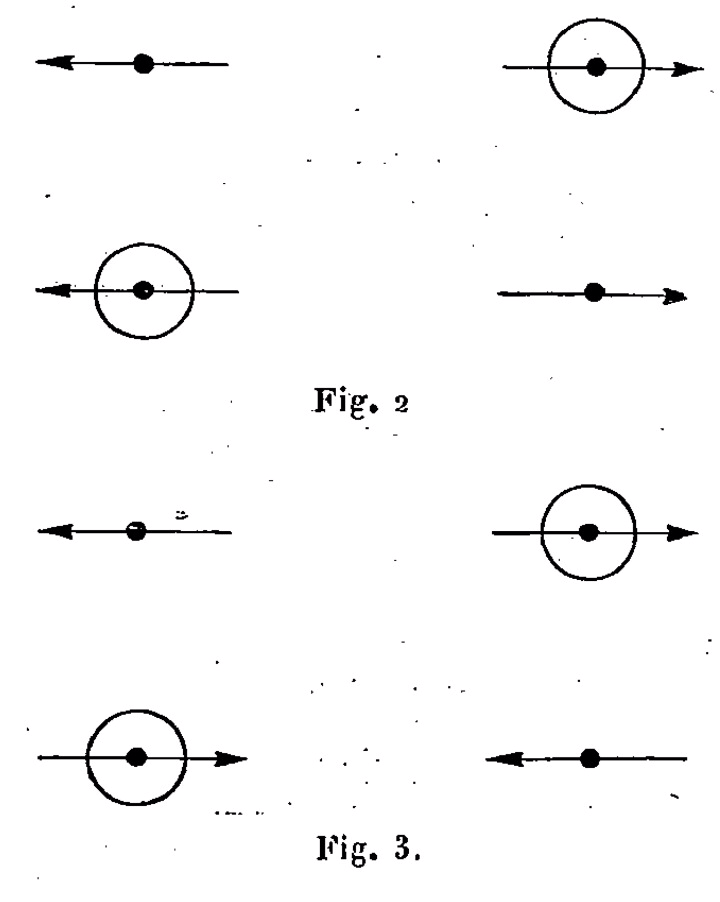
\includegraphics[width=200pt]{images/Fig2Fig3}
\end{figure}

and with the representation 1 you get:
\nequ{10}{
\mathcal{J}(r_{kl})\frac{1}{2}\left[\rho_k^\xi \rho_l^\xi + 
\rho_k^\eta \rho_l^\eta \right]
}
or, with representation 2:
\nequ{11}{
-\mathcal{J}(r_{Kl})\cdot P'_{Kl}
}
where $P'_{Kl}$ 
represents the operator that permutes the variables $r_K,\sigma_K$ with $r_l,\sigma_l$.

The exchange action introduced by Majorana and which will be discussed later (it is represented schematically in figure 3) on the contrary leads to terms in the Hamiltonian which are written in representation 1
\nequ{12}{
\mathcal{J}(r_{kl})\frac{1}{4} \left[\rho_k^\xi \rho_l^\xi + 
\rho_k^\xi  \rho_l^\eta \right]\left[1+(\sigma_k\sigma_l)\right],
}
and in representation 2
\nequ{13}{
-\mathcal{J}(r_{Kl})P_{Kl},
}
where $P_{Kl}$ is the operator corresponding to a permutation of the space coordinates $r_K$and $r_l$.

To reduce the number of possible hypotheses for the exchange action, Majorana\footnote{\citeauthor{E. Majorana}, \citepub{Zeits. f. Phys.}, \citevol{82}, \citeyear{1933}, \citepage{p. 137}} has leaned on the simplest experimental facts. One of the most characteristic traits of the nuclear structure is that the nuclear radius seemingly varies as the cube root of the mass (see \S2,a), that is to say that the density of nuclear matter appears to be basically independent of its value. This suggests that the nucleus is not, like the atom itself, a central system on the interior of which a particular point plays the role of a center of force, but on the contrary presents analogy with the liquid state, and hence as we have indicated apropos Gamow's drop model, where the size of the drop has no influence on the conditions in which a new molecule is added. The theory of liquids shows that the existence of a finite molecular radius and the presence of mutual actions of the Van der Waals type form the essential bases of a representation of the liquid state. In the same manner, the experimental properties of the nucleus can only be represented in the hypothesis of ordinary forces between protons and neutrons if one introduces a finite radius for the neutron, that is to say a minimum distance below which there appears an important repulsive force between the proton and the neutron. This consequence, difficult to accept, may be avoided by introducing an exchange action between protons and neutrons. If fact, as has been shown in London and Heitler's theory of molecules, these exchange actions give rise to a \?{saturation of bonds}{saturation des liaisons}, which leads to results analogous to the hypothesis of a finite neutron radius. Such a saturation occurs when the sign of $J(r_{Kl})$ in the equations (10) to (13) is positive. The mathematical development will be found later.

Majorana legitimately draws the conclusion — in opposition to one of the author's earlier reports — that, for experimental reasons, the positive sign is the most likely for $J(r_{Kl})$. An additional argument in favor of (12), (13) against (10), (11) results from the fact that in this latter conception the nucleus $\mnEl{2}{1}{H}$ here represents a closed system, whereas in the action of forces represented by (12), (13) this saturation only appears in the helium nucleus.

We now indicate the mathematical justification of these results.  Following Majorana's example, we apply the Thomas-Fermi method to a nucleus composed of a large number of particles in the form given by Dirac. With Majorana, we choose the second of the mathematical representations indicated on page 301. In these conditions, the Schr\"odinger function for a nucleus composed of $n_1$ neutrons and $n_2$ protons may be written to first approximation in the form
\uequ{
\Phi = \left|\begin{matrix}
\varphi_{1}\left(\vec{r}_I, \sigma_I\right) & \dots &
\varphi_{n_1}\left(\vec{r}_I, \sigma_I\right)\\
\varphi_{1}\left(\vec{r}_{II}, \sigma_{II}\right) & \dots &
\varphi_{n_1}\left(\vec{r}_{II}, \sigma_{II}\right)\\
\dots\dots & \dots & \dots\dots\\
\varphi_{1}\left(\vec{r}_{n_1}, \sigma_{n_1}\right) & \dots &
\varphi_{n_1}\left(\vec{r}_{n_1}, \sigma_{n_1}\right)\\
\end{matrix}
\right|
\left|\begin{matrix}
\varphi_{1}\left(\vec{r}_I, \sigma_I\right) & \dots &
\varphi_{n_2}\left(\vec{r}_I, \sigma_I\right)\\
\varphi_{1}\left(\vec{r}_{II}, \sigma_{II}\right) & \dots &
\varphi_{n_2}\left(\vec{r}_{II}, \sigma_{II}\right)\\
\dots\dots & \dots & \dots\dots\\
\varphi_{1}\left(\vec{r}_{n_2}, \sigma_{n_2}\right) & \dots &
\varphi_{n_2}\left(\vec{r}_{n_2}, \sigma_{n_2}\right)\\
\end{matrix}
\right|.
}

The total potential energy corresponding to $\Phi$ for the exchange actions (13) becomes:
\nequ{15}{
E_\text{pot} = -&\int\Phi^*\sum\limits_{K,k}\mathcal{J}(r_{K,k})P_{K,k}\Phi d\omega\\
= &\sum\limits_{\sigma\sigma'}\int\int d\vec{r}d\vec{r}'
\sum\limits_{K=1}^{n_1}\varphi_K^*\left(\vec{r},\sigma\right)
\varphi_K\left(\vec{r}',\sigma\right)\\
\times & \sum\limits_{k=1}^{n_2}\varphi_k^*\left(\vec{r}',\sigma'\right)
\varphi_k\left(\vec{r}',\sigma'\right)
\mathcal{J}\left(\vec{r} - \vec{r}'\right).
}

Ignoring the actions exerted by the spin of the particles and consequently writing $\varphi_K\left(\vec{r},\sigma\right)$ as $\chi_K(\vec{r})f_K(\sigma)$, the equation (15) takes the form
\nequ{16}{
E_\text{pot} = -\int\int d\vec{r} d\vec{r}' \sum\limits_{K=1}^{n_1}\chi_K^*(\vec{r})\chi_K(\vec{r}')\mathcal{J}\left(\left|\vec{r}-\vec{r}'\right|\right)\sum\limits_{k=1}^{n_1}\chi_k^*(\vec{r}')\chi_k(\vec{r}).
}

The expressions
\nequ{17}{
\rho_N(\vec{r}) = \sum\limits_{K=1}^{n_1}\chi_K^*\chi_K,\\
\rho_P(\vec{r}) = \sum\limits_{k=1}^{n_1}\chi_k^*\chi_k,\\
}
which respectively represent the density of the neutrons and of the protons, are replaced as is well-known in the Thomas-Fermi method by
\nequ{18}{
\rho_N(\vec{r}) = \frac{2}{h^2}\int_0^{p_N(\vec{r})}d\vec{p},\quad
\rho_P(\vec{r}) = \frac{2}{h^2}\int_0^{p_P(\vec{r})}d\vec{p},
}
where the limits $p_N$ and $p_P$ are determined by the potential energy at the point $r$. In an analogous manner, we write with Dirac\footnote{\citeauthor{P.A.M. Dirac},\citepub{Proc. Cambr. Phil. Soc.}\citevol{26}\citeyear{1930}\citepage{p. 376}}:
\nequ{19}{
\sum\limits_{K=1}^{n_1}\chi_K^*(\vec{r})\chi_K(\vec{r}') = & \rho_N\left(\vec{r}, \vec{r}'\right) = \frac{2}{h^3}\int_0^{p_N\left(\frac{r+r'}{2}\right)}d\vec{p}\,\,
\exp{\frac{i}{h}\vec{p}\left(\vec{r}'-\vec{r}\right)}\\
& \rho_P\left(\vec{r}, \vec{r}'\right) = \frac{2}{h^3}\int_0^{p_P\left(\frac{r+r'}{2}\right)}d\vec{p}\,\,
\exp{\frac{i}{\hbar}\vec{p}\left(\vec{r}'-\vec{r}\right)},
}
which results in
\nequ{20}{
E_\text{pot} = -\int\int d\vec{r}\,d\vec{r}'\frac{4}{h^6}\int\limits_0^{p_N}d\vec{p}\int\limits_0^{p_P}d\vec{p}'\,\,
\exp{\frac{i}{\hbar}\left(\vec{p} - \vec{p}'\right)\left(\vec{r}' - \vec{r}\right)}\mathcal{J}\left(\left|\vec{r}'-\vec{r}\right|\right).
}
As elsewhere $\rho_N\left(\vec{r}, \vec{r}'\right)$ and $\rho_P\left(\vec{r}, \vec{r}'\right)$ are only different from zero in a small interval around $\left(\vec{r}' - \vec{r}\right) = 0$, or when the particle density is large, and as, in addition, for the majority of nuclei $p_N>p_P$, that is to say $\rho_N>\rho_P$, equation (20) can be given the following form if $J\left(\left|\vec{r}'-\vec{r}\right|\right)$ varies \?{monotonically}{régulièrement} with $\left|\vec{r}'-\vec{r}\right|$ and more slowly than $\rho_N\left(\vec{r}, \vec{r}'\right)$ around the point $\left(\vec{r}-\vec{r}'\right)=0$:
\nequ{21}{
E_\text{pot} \approx -2\int d\vec{r}\,\,\rho(\vec{r})\mathcal{J}(0) = -2n_2 \mathcal{J}(0).
}

This rough approximation is not however sufficient for determining $\rho_N$ and $\rho_P$ in a given nucleus. To obtain a better approximation one may, thanks to the rapid variation of $\rho_N(\vec{r}, \vec{r}')$ with $(\vec{r} - \vec{r}')$, replace equation (20) by
\nequ{$21^\text{a}$}{
E_\text{pot} &\approx -\int d\vec{r} \int d\vec{s}\,\frac{4}{h^6}
\int\limits_0^{(p_N r)}d\vec{p} \int\limits_0^{p_P(r)}d\vec{p}'\,\,
\exp{\frac{i}{\hbar}(\vec{p} - \vec{p}')\vec{s}}\mathcal{J}(|s|)\\
&= -\int d\vec{r}\,\,f\left[\rho_N(\vec{r}), \rho_P(\vec{r})\right],
}
where $f$ is a function that is symmetric in $\rho_N$ and $\rho_P$, which vanishes with $\rho_N$ or $\rho_P$ and which tends, for large densities, to the limits $2\rho_N J(0)$ or $2\rho_P J(0)$ according to whether one has $\rho_N < \rho_P$ or $\rho_N > \rho_P$.

Since the other part of the kinetic energy, according to Thomas and Fermi, is given by
\uequ{
E_\text{kin} = \frac{h^2}{M}\frac{4\pi}{5}\left(\frac{3}{8\pi}\right)^\frac{5}{3}
\int d\vec{r}\left(\rho_N^\frac{5}{3} + \rho_P^\frac{5}{3}\right),
}
the result is
\nequ{22}{
E = \int d\vec{r}\left[\frac{h^2}{M}\frac{4\pi}{5}
\left(\frac{3}{8\pi}\right)^\frac{5}{3}
\left(\rho_N^\frac{5}{3} + \rho_P^\frac{5}{3}\right)
 - f(\rho_N, \rho_P)\right].
}
The functions $\rho_N(\vec{r})$ and $\rho_P(\vec{r})$ are obtained \?{by varying}{en faisant varier} $\rho_N$ or $\rho_P$ in $E$ under the conditions
\nequ{23}{
n_1 = \int\rho_N vec{r}, \quad n_2 = \int\rho_P d\vec{r}.
}

As a result
\uequ{
\rho_N(\vec{r}) = \text{const.} = c_1,\quad
\rho_P(\vec{r}) = \text{const.} = c_2.
}
If $V$ is the volume of the nucleus, one has
\uequ{
c_1 = \frac{n_1}{V},\quad
c_2 = \frac{n_2}{V}
}
and consequently
\nequ{24}{
E = \frac{h^2}{M}\frac{4\pi}{5}\left(\frac{3}{8\pi}\right)^\frac{5}{3}
\left(n_1^\frac{5}{3} + n_2^\frac{5}{3}\right)V^{-\frac{2}{3}}
 - Vf\left(\frac{n_1}{V}, \frac{n_2}{V}\right)
}
and from $\dXdY{E}{V} = 0$:
\nequ{25}{
-\frac{h^2}{M}\frac{8\pi}{15}\left(\frac{3}{8\pi}\right)^\frac{5}{3}
\left[\left(\frac{n_1}{V}\right)^\frac{5}{3} + \left(\frac{n_2}{V}\right)^\frac{5}{3}\right]\\
- f\left(\frac{n_1}{V}, \frac{n_2}{V}\right) + \frac{n_1}{V}\pXpY{f}{\rho_N}
+ \frac{n_2}{V}\pXpY{f}{\rho_P} = 0,
}
\?{the condition which determines the volume of the nucleus}{condition qui détermine le volume du noyau}. If the ratio $\frac{n_1}{n_2}$ is kept constant, it follows from (25) that the volume of the nucleus varies proportionally with the mass. This demonstrates that the exchange interaction introduced by Majorana leads, for the nuclear matter, to characteristics analogous to those of a liquid. Moreover, the saturation indicated earlier for the bonding forces results here from equation (21) according to which the exchange action of a proton may only be exerted on average on two neutrons.

After this result it is seen why a helium nucleus \?{appears as}{présente l'aspect de} a closed system. By virtue of the Pauli principle, there is only room for two neutrons or two protons in the same state. Neutrons in a well-defined state may be bound to a proton, the total binding energy being proportional to their number. Neutrons in other states on average do not provide any contribution to the binding energy. Imagining the nuclei as constructed by successive \?{blocks}{apports} of neutrons and protons, a new closed system must be constituted each time that two new protons and two new neutrons have been added, which may be considered as corresponding to the formation of a new helium particle.

Despite the insufficiency of the indicated procedure, one may try to deduce in a qualitative manner the variation of the mass defect with $J(r)$, $n_1$ and $n_2$. It may be used, in view of the last application, to pursue the consequences of a particularly simple hypothesis on the form of $J(r)$ and to calculate the corresponding form for the function $f(\rho_l, \rho_P)$.

To the form proposed by Majorana
\nequ{27}{
\mathcal{J}(r) = a\exp{-br}
}
corresponds, according to (21):
\nequ{28}{
f(\rho_N, \rho_P) = a\frac{b^3}{6\pi^3}\left\{4NP +
\left[1 + 3(N^2+P^2)\right]
\log{\frac{1+(N-P)^2}{1+(N+P)^2}}\right.\\
+ 4(N^3+P^3)\arctan{(N+P)}\\ \left.
- 4(N^3-P^3)\arctan{(N-P)}\right\}
}
where we have put
\uequ{
N=\frac{1}{b}\sqrt[3]{3\rho_N \pi^2}\quad
\text{ and }\quad
P=\frac{1}{b}\sqrt[3]{3\rho_P \pi^2}.
}

According to whether $a$ is
\uequ{
\ll \frac{\hbar^2 b^2}{M}
\quad\text{ or }\quad
\gg \frac{\hbar^2 b^2}{M}
}
one will have, according to (25),
\uequ{
N \text{ and } P \ll 1 \text { or } \gg 1
}

Consequently, for the statistical method to give usable results, it is necessary to suppose that
\uequ{
a \gg \frac{\hbar^2 b^2}{M}.
}

If this condition is fulfilled, the expression (28) may be approximately replaced by
\nequ{29}{
f=a\frac{b^3}{3\pi^3}\left\{\pi(N^2 + P^2) - 2(N-P)^2\right.\\
- \frac{3}{2}(N^2 + P^2)\log{\frac{(N+P)^2}{1+(N-P)^2}}\\
\left. - 2(N^3-P^3)\arctan{(N-P)}\right\}.
}

These calculations must be modified in the case of heavy nuclei to take account of the Coulomb force. In place of (22) one obtains the equation
\nequ{30}{
E = \int d\vec{r}\left\{\frac{h^2}{M}\frac{4\pi}{5}\left(\frac{3}{8\pi}\right)^\frac{5}{3}\left(\rho_N^\frac{5}{3} + \rho_P^\frac{5}{3}\right) - f(\rho_N, \rho_P)\right\}\\
+ \frac{1}{2}\int\int d\vec{r}\,\,d\vec{r}'\frac{e^2}{|r-r'|}\rho_P(\vec{r})\rho_P(\vec{r}').
}

Varying $\rho_N$ and $\rho_P$ in $E$ one obtains equations which transform via the ordinary Thomas-Fermi method into differential equations for $\rho_N$ and $\rho_P$. Under the influence of the Coulomb forces, the densities $\rho_N$ and $\rho_P$ vary on the interior of the nucleus, these Coulomb forces tending to accumulate the positive charge on the external surface. As long as the influence of these forces remains weak, that is to say for nuclei that are not too heavy, we may treat their action as small perturbations and for calculating the mass defects, introduce the unperturbed densities in the \WTF{complementary term} of (30). The Coulomb term in the energy then becomes:
\nequ{31}{
\iint d\vec{r}\, d\vec{r}' \frac{e^2}{|\vec{r} - \vec{r}'|}
\rho_P(\vec{r})\rho_P(\vec{r}) = \frac{3}{5}(n_2 e)^2
\left(\frac{3V}{4\pi}\right)^{-\frac{1}{3}}.
}

In the following chapter we compare the formulae obtained in this way with the experimental data.

\subsection{General consequences for the table of isotopes.}

The hypotheses on the structure of the nucleus which have been developed in parts a b c of section 2 permit drawing certain general conclusions on the particularities of the table of isotopes and the laws of radioactive decay.

The various ideas all lead to the result that the properties of the nucleus, such as stability, abundance in nature, spin, etc, present a certain periodicity on a variation of 4 in the mass and 2 of the charge, which is well-confirmed by experiment in a general manner. The Gamow model and the 2nd scheme lead in particular to a very marked influence of the mass on the properties of the nucleus, according to which this mass is of the form $4n$, $4n+1$,$4n+2$ or $4n+3$. On the contrary, the charge of the nucleus for a given mass and in particular the fact that this charge is either even or odd does not seem to play as important a role. To the extent that one may speak of the properties of nuclear electrons, experiment seems to indicate that they follow Bose statistics; thus one should not predict a periodicity on a variation of 2 of the charge. If on the other hand the nucleus is considered to be composed of neutrons and protons (schemas 3 and 4), one must predict in the first place a periodicity of the nuclear properties on a variation of 2 in the charge, \?{since one always has at least as many neutrons as protons}{puisqu’on a toujours en présence au moins autant de neutrons que de protons}, and two new elementary charges are always sufficient for the formation of an $\alpha$ particle; in the second place for a given charge a rather less marked periodicity of variation 2 in the mass by applying the Pauli principle to the proton and to the neutron. In the sense of the periodicity predicted by schemas 3 and 4, one must predict for example the analogies between the nuclei $\mnEl{124}{54}{Xe}$, $\mnEl{126}{54}{Xe}$, $\mnEl{128}{54}{Xe}$, $\mnEl{130}{54}{Xe}$ and $\mnEl{132}{54}{Xe}$ while the periodicity that results from Gamow's scheme must predict for common characteristics for the nuclei $\mnEl{124}{54}{Xe}$, $\mnEl{128}{54}{Xe}$ and $\mnEl{132}{54}{Xe}$ not appearing in the nuclei $\mnEl{126}{54}{Xe}$ and $\mnEl{130}{54}{Xe}$.
\begin{figure}[h!]
\centering
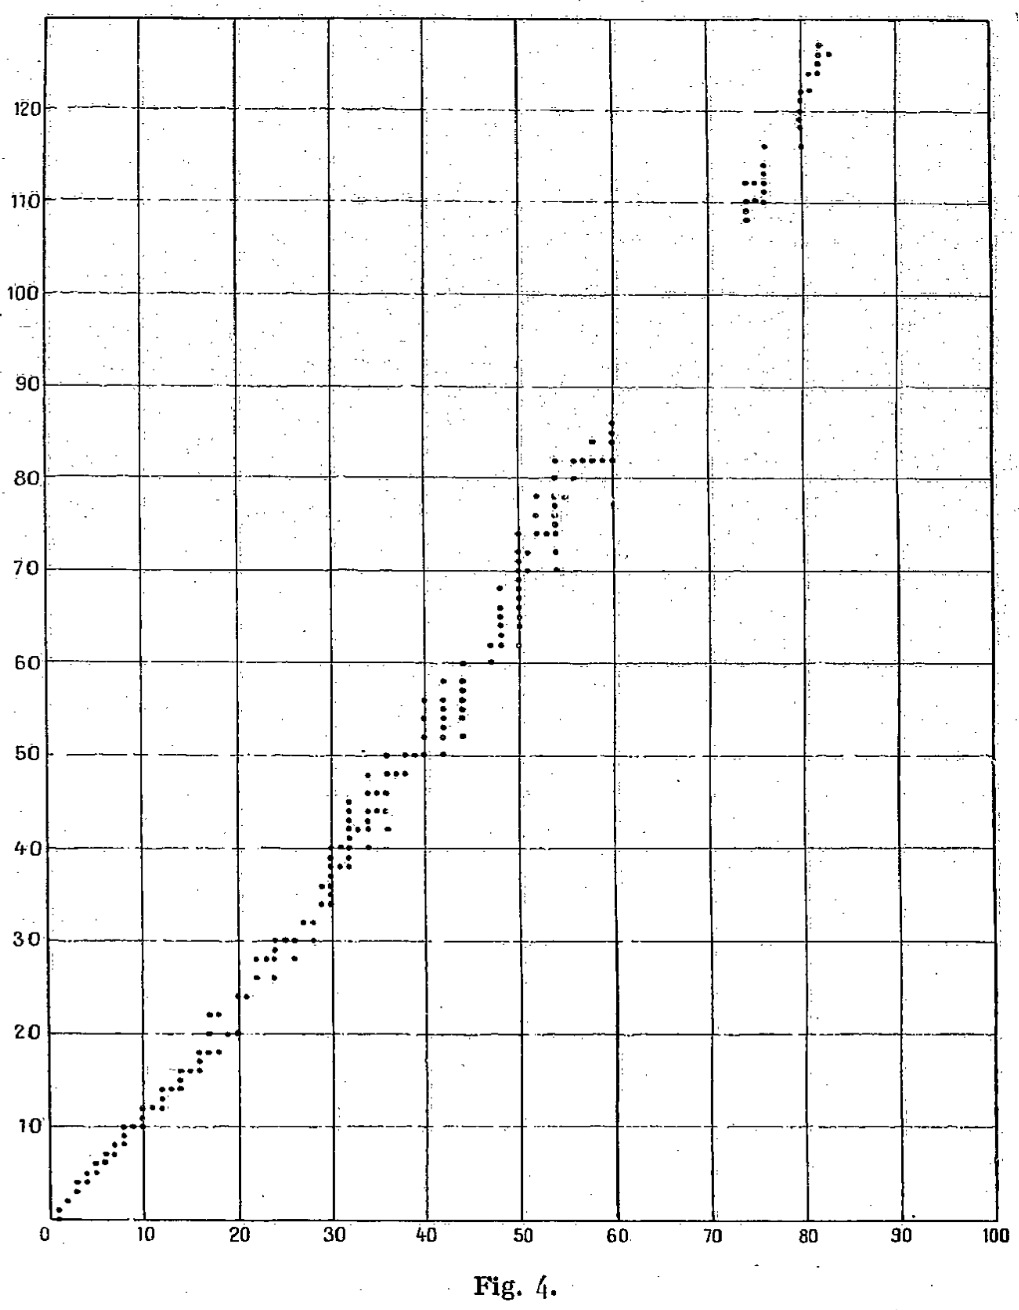
\includegraphics[width=350pt]{images/fig4}
\end{figure}
In figure 4 the known nuclei are represented by arraying the number of protons $n_2$ on the $x$-axis and the number of neutrons $n_1$ on the $y$-axis, where each nucleus corresponds to one nucleus. The table obtained in this way nicely indicates a predominance of even charge and, in a less marked manner, a predominance of even numbers of neutrons. This observation, though it is not in contradiction with Gamow's scheme, supplies an argument in favor of hypotheses 3 or 4 since they can be predicted by this hypothesis.

\begin{figure}[h!]
\centering
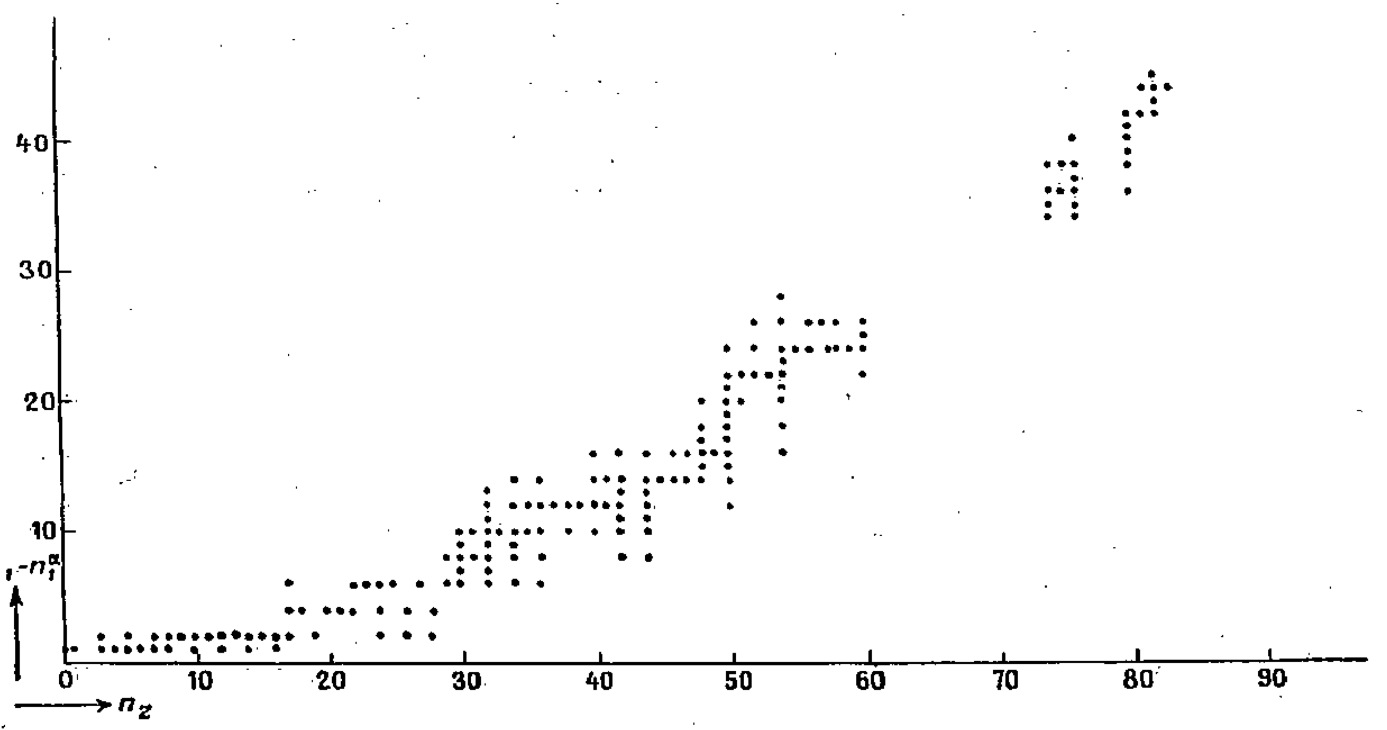
\includegraphics[width=300pt]{images/Fig5}
\end{figure}

In this conception, the nucleus is constructed from neutrons and protons in the following manner: each time two protons and two neutrons have been added, a new shell is completed by the formation of a helium atom. For nuclei which only contain $\alpha$ particles, it is not necessary to assume the formation of any shell beyond this construction of helium nuclei; in fact, the large \?{formation energy}{énergie de formation} of the $\alpha$ particle permits considering them to a certain extent as \?{the building blocks}{des éléments constitutifs} of the nucleus, and the fact that they follow Bose statistics has as a consequence that they are all placed on the lowest energy level. It is otherwise, a fact which Landé\footnote{\citeauthor{A. Landé}, \citepub{Phys. Rev.}, \citevol{43}, \citepage{pp. 620 and 624}.} has justly insisted upon, for neutrons which do not join in an $\alpha$ particle. If one assumes a nucleus constructed from $\alpha$ particles, neutrons, and eventually a proton makes it possible to obtain a good approximation for the solution to the already-complicated quantum-mechanical problem which concerns the heavy nuclei, one may compare the motion of the neutrons in the field of action of the $\alpha$ particles with that of the peripheral electrons in the field which surrounds the atom, and thus one may expect a structure of successive shells for this system of neutrons. Landé has depicted, in figure 5, the experimental number of neutrons independent of the $\alpha$ particles for various atomic numbers, and he considers that this figure leads immediately to the following interpretation: until the charge $n_2=16$, only the lowest level of the system of neutrons is occupied and may constitute a shell of two neutrons; between $n_2 = 17$ and $n_2=18$ this shell must always be complete and a subsequent shell of four neutrons may be completed; from $n_2=32$ up to $n_2=36$ a subsequent shell of eight is completed, and so forth. If on the other hand one seeks to predict theoretically the formation of successive shells, one must first of all examine the possible stationary states of the field inside the nucleus.  The potential distribution which determines the motion of a neutron inside the nucleus is known qualitatively. The density of $\alpha$ particles must be approximately constant inside the nucleus with a slight increase towards the surface because of the Coulomb action. Consequently there is for the neutron a variation of the potential of the form depicted in figure 6.
\begin{figure}[h!]
\centering
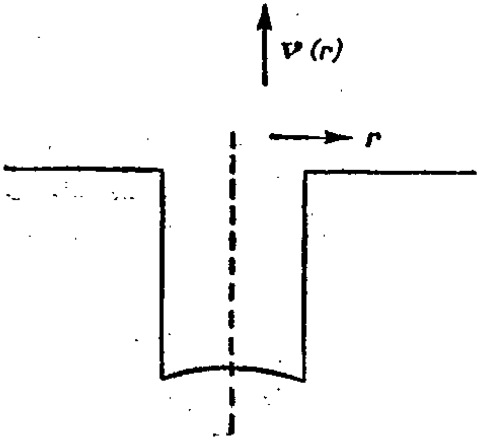
\includegraphics[width=150pt]{images/Fig6}
\end{figure}
The states of weaker energy which correspond to this potential represent, ignoring the reaction of the spin on the \WTF{moment of circulation}, an $S$-term ($l=0$), a $P$-term ($l=1$) and a $D$-term ($l-2$) (\textit{cf.} Gamow's report, \textit{fig. 10}). Adding a hypothesis of a spin reaction, one will obtain for the lowest terms a picture analogous to that of figure 7. According to this arrangement, one would obtain first a shell of two, and then one of four neutrons (appearance of the term $j=\frac{3}{2}$), then again one of two, one of six, one of four, etc. It is not yet possible to grasp how far a similar arrangement constructed from orbits of individual neutrons permits taking account of the experimental facts concerning the system of isotopes.
\begin{figure}[h!]
\centering
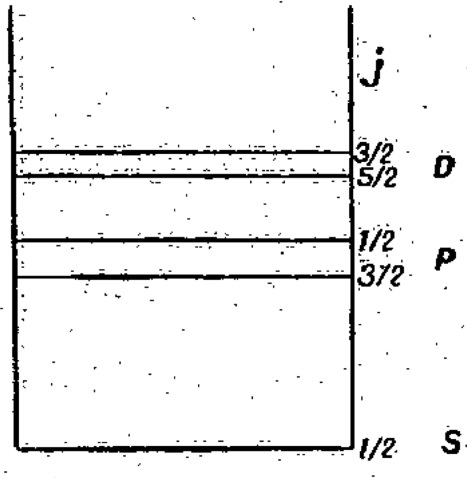
\includegraphics[width=150pt]{images/Fig7}
\end{figure}
The question of the stability of the nucleus from the $\alpha$ decay point of view is completely elucidated by the theory of Gamow, Condon and Gurney (\textit{cf.} Gamow's report); Gamow's theory applies moreover in an analogous manner to various nuclear models. As this theory makes the stability of the nucleus, from the $\alpha$ decay point of view, depend uniquely on the balance of energy of this process, it may be assumed that, for a nucleus of a given mass, the Coulomb forces make the decay all the more probable as the charge of the nucleus increases. The fact that there is, for a given mass, an experimental upper bound on the charge at just below half the atomic mass leads naturally to the hypothesis that strongly-charged nuclei dissociate by emitting $\alpha$ particles. Moreover it is seen that, among radioactive nuclei of the same mass, it is in general those of higher charge which manifest the larger decay energy.

It is currently difficult to treat in a satisfactory manner the question of the stability of a nucleus to $\beta$ decay. In Gamow's primitive theory, the energy balance determines the stability from the point of view of the emission of a $\beta$ ray as well as from an $\alpha$ ray. This idea is not easily justified, since it is an experimental fact that the $\beta$ particles emitted by the nucleus are distributed with a continuous energy spectrum and there does not seem to be any relation between the mean decay energy and the mean lifetime for $\beta$ decay analogous to that of Geiger-Nuttall for $\alpha$ decay. However, this question remains open, since the existence of a well-defined upper bound on the continuous $\beta$ spectrum represents a difficulty for all theories based on the principle that the $\beta$ particles are emitted by the nucleus with an indeterminate energy. Pauli has examined the hypothesis that the emission of $\beta$ rays are always accompanied by a very penetrating radiation consisting for example of a "neutrino" with mass equal to that of an electron, which would permit maintaining conservation of energy in the case of $\beta$ decay. Bohr\footnote{\citeauthor{N. Bohr}, \textit{loc. cit.}} on the other hand considers it more likely that $\beta$ emission by the nucleus is an exception to the principle of conservation of energy.

The theoretical aspect of this question of $\beta$ decay is not modified if one considers the nucleus as constituted of protons and neutrons. In this case, the question of stability with respect to a $\beta$ decay is reduced to knowing if a neutron can dissociate into a proton and an electron when it is found in a force field energetically favorable to this decomposition. For the solution of this problem we must, for the reasons indicated above, we must content ourselves with experimental observations. If the energy balance determines $\beta$ stability, there must be an upper bound on the mass for each nuclear charge beyond which the nucleus dissociates and emits an electron. It is consequently useful to establish the energy balance for $\beta$ decay starting from the mass defects, to the extent they are known empirically or theoretically, and comparing the results with the table of nuclei known to be stable. We give the results of this comparison apropos the application of Majorana's formula.

Considering the $\beta$ decay as determined by the energy balance, the ideas 3-4 give a satisfactory interpretation of the fact that $\beta$ emission from a nucleus of even charge always leads to consecutive couples. If, in fact, the energetic conditions are favorable to the emission of a primary $\beta$ particle, a second emission, after which a new $\alpha$ particle may be formed in the nucleus, would find energetic conditions at least as favorable\footnote{\citeauthor{Heisenberg}, \citepub{Zeits. f. Phys.}, \citevol{77}, \citeyear{1932}, \citepage{p. 1}; \citevol{78}, \citeyear{1932}, \citepage{p. 156}; \citevol{80}, \citeyear{1933}, \citepage{p. 587}.}. It is only for an initially-odd nuclear charge that a single $\beta$ particle may eventually be emitted \WTF{(Ac)}. The fact that there are no stable nuclei beyond $\mnEl{7}{14}{N}$ with odd numbers of protons and neutrons may in the same manner receive a simple energetic interpretation.

\section{Applications.}
\subsection{Mass defect and stability of nuclei.}

Very precise indications on the subject of the mass defect are obtained starting from hypotheses on the structure of the nucleus corresponding to arrangements 3-4, in particular taking the point of view of Majorana, which may be considered as corresponding to a form of Gamow's drop model, sharpened with the neutron hypothesis. One may attempt to determine the two constants in the force law introduced as an example: $J(r) = a\exp{-br}$ in a way so that the mass defects of the two nuclei are conveniently chosen to be exactly represented by equation (30), and see how the mass defects calculated for other nuclei with this formula \?{fall}{se placent} with respect to d'Aston's experimental curve. In this comparison it must be remembered that the Thomas-Fermi method used for obtaining equation (30) may not give exact results for light nuclei. This equation must however qualitatively represent the mass defects for various nuclei beyond $n=20$, for example, though it must give a too-high absolute value for binding energy, since this energy per particle is certainly much weaker for the very light nuclei than for heavy nuclei. Adding a constant term to the second part of (30), one might get closer to reality.

Putting for example in $J=a\exp{-br}$:
\uequ{
a &= Mc^2 \times 0.0273 = 4.05\cdot 10^{-5}\text{erg},\\
b &= \frac{Mc}{h} \times 0.165 = 1.25\cdot 10^{12} \text{cm}^{-1},
}
after some calculations, one deduces from these equations and (31) the \?{approximate}{approchée}:
\nequ{33}{
\frac{E}{Mc^2} = 0.00347n_2 - 0.0364n_1 + 0.01211 \frac{n_1^2}{n_2}\\
+ n_2^\frac{5}{3}\left(3.19 - 0.715\frac{n_1}{n_2}\right)\cdot 10^{-4}(+0.049).
}

The first line represents the influence of exchange actions, the second the repulsive Coulomb action between the protons and the additive term just mentioned and which is not contained in equation (30); this term is chosen to reproduce d'Aston's values as well as possible. Figure 8 gives the result of the comparison of the values thus calculated with d'Aston's measurements, the mass of the neutron having been, for this comparison, supposed to be equal to that of the proton.

One must not attribute too great a significance to the relatively-good agreement that results from this comparison since, for establishing the formula (33), the three arbitrary constants have been disposed and that, on the other hand, as insisted by Majorana and as we have indicated earlier, the application of the Thomas-Fermi method may include important errors, even for high-enough numbers of particles. One may however conclude that the formula (30) gives, at least qualitatively, the correct variation of the energy with $n_1$ and $n_2$.
\begin{figure}[h!]
\centering
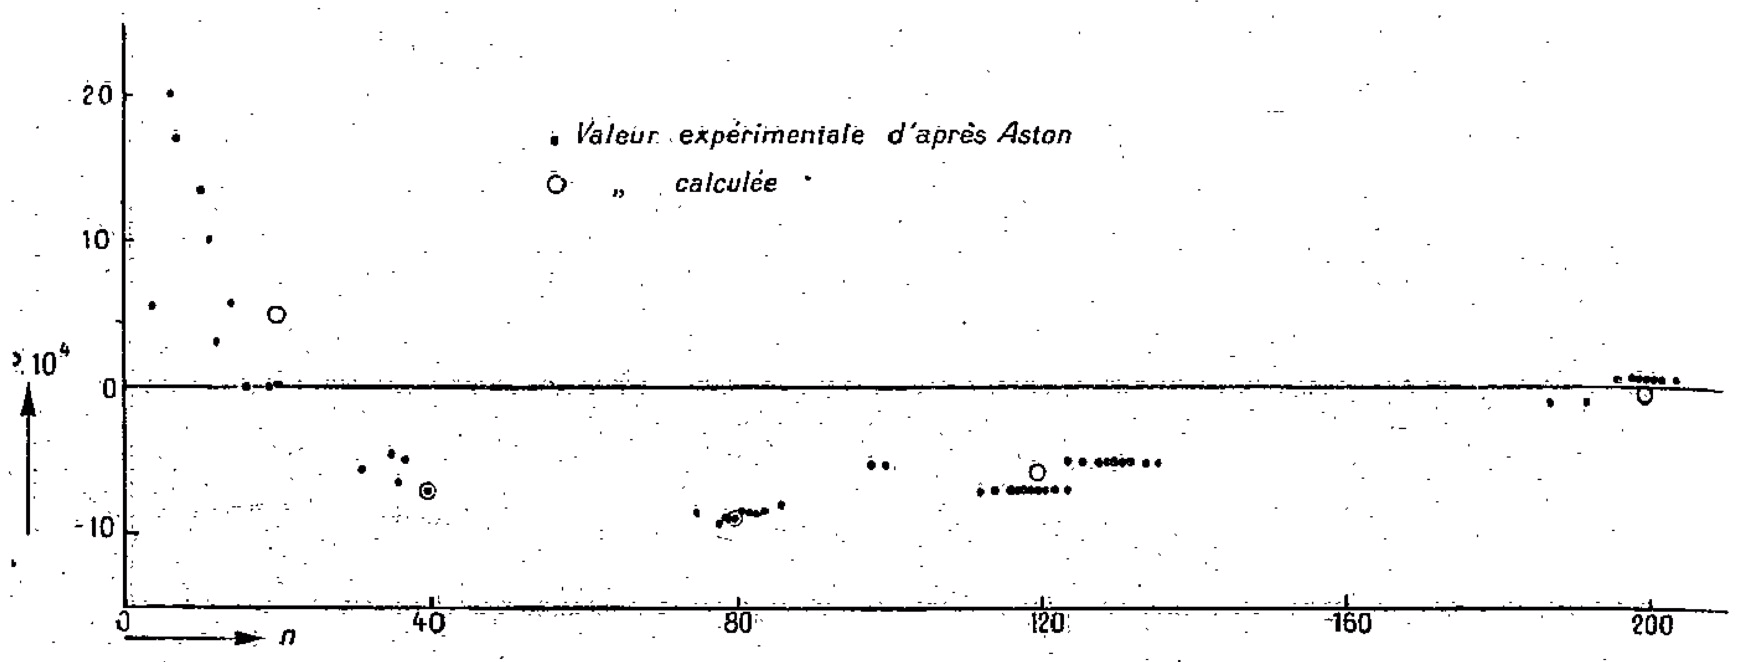
\includegraphics[width=300pt]{images/Fig8}
\end{figure}
A greater importance can be attached to the consequences which may be deduced from equations (30) and (33) concerning the stability of the atomic nucleus. The energy necessary to extract two protons and two neutrons from the nucleus is given according to (33), in \WTF{fractions of the intrinsic energy of the proton}, by
\nequ{34}{
-2\left(\pXpY{E}{n_1} + \pXpY{E}{n_2}\right) = 0.0658 - 0.04844\frac{n_1}{n_2} + 0.02422\left(\frac{n_1}{n_2}\right)^2\\
+\left(9.2 - 0.954\frac{n_1}{n_2}\right)n_2^\frac{3}{2}\cdot 10^{-4}.
}

If this energy is larger than the binding energy of a helium nucleus, the nucleus under consideration is stable with respect to decay; if on the contrary it is smaller, it may spontaneously emit an $\alpha$ particle.

In figure 9 the curves of constant decay energy are traced by taking the experimental value of the $\alpha$ particle's mass defect and assuming the neutron's mass defect from a proton and an electron is negligible.

One of these curves, the one corresponding to $\Delta E = 0$, represents the boundary between the stable and unstable atomic nuclei. If you plot on this figure the points corresponding to experimentally stable atomic nuclei, it is found that the lower limit of these points are in general in good agreement with the curve of null decay energy; the curve $\Delta E = -0.003$ would fit better than $\Delta E=0$, but but given the arbitrarily-made approximations (neutron mass equal to that of the proton, etc), these results may not be invoked against the validity of the formula (30).

The energy difference between the initial and final states of a $\beta$ decay process can be calculated in the same manner:
\nequ{35}{
\pXpY{E}{n_1} - \pXpY{E}{n_2} = -0.0399 + 0.02422\frac{n_1}{n_2}
+ 0.01211\left(\frac{n_1}{n_2}\right)^2\\
- \left(6.04 - 0.477\frac{n_1}{n_2}\right)n_2^\frac{2}{3}\cdot 10^{-4}.
}
\begin{figure}[h!]
\centering
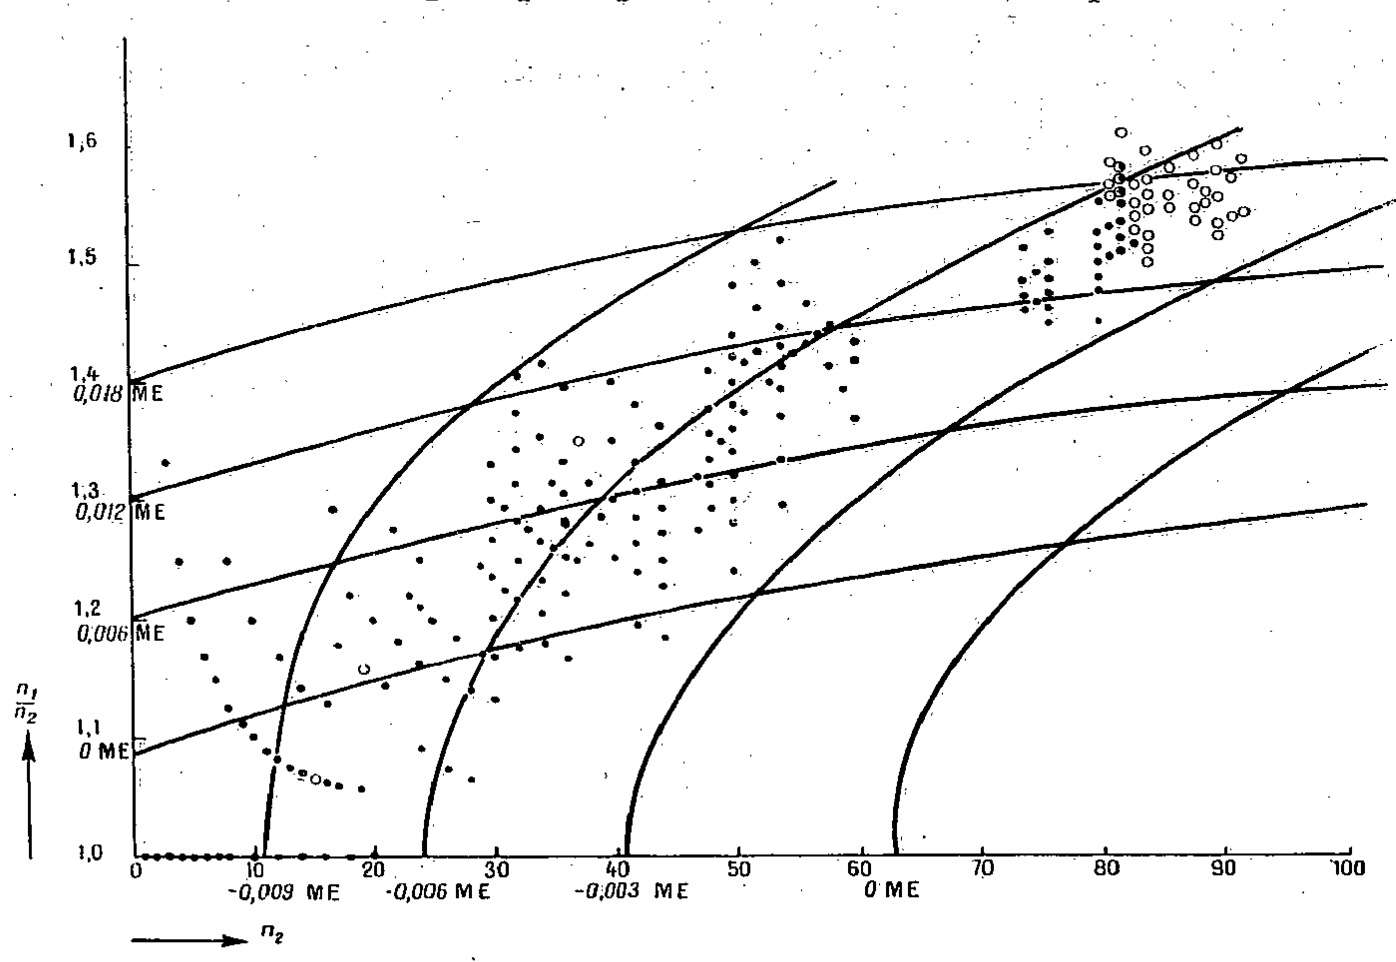
\includegraphics[width=300pt]{images/Fig9}
\end{figure}
The curves of constant decay energy (\textit{fig. 9}) found here are almost parallel to the upper bound of the points corresponding to stable atomic nuclei, and this represents an argument in favor of an energetic stability criterion from the point of view of $\beta$ emission. The $\Delta E = 0$ curve is again noticeably too low. However it may be remarked that, for $\alpha$ decay as well as $\beta$, the $\Delta E=0$ curve may not exactly represent the limit of experimentally unstable atomic nuclei. In fact, it is a result of Gamow's theory for decay that heavy atomic nuclei, even when they can emit an $\alpha$ particle with a kinetic energy of $5\cdot 10^{-6} \text{erg}$ behave as if they were practically stable because of their long mean lifetime; analogous circumstances are probably present in the case of $\beta$ emissions\footnote{\textit{See} the note at the finish of this report.}.
\begin{figure}[h!]
\centering
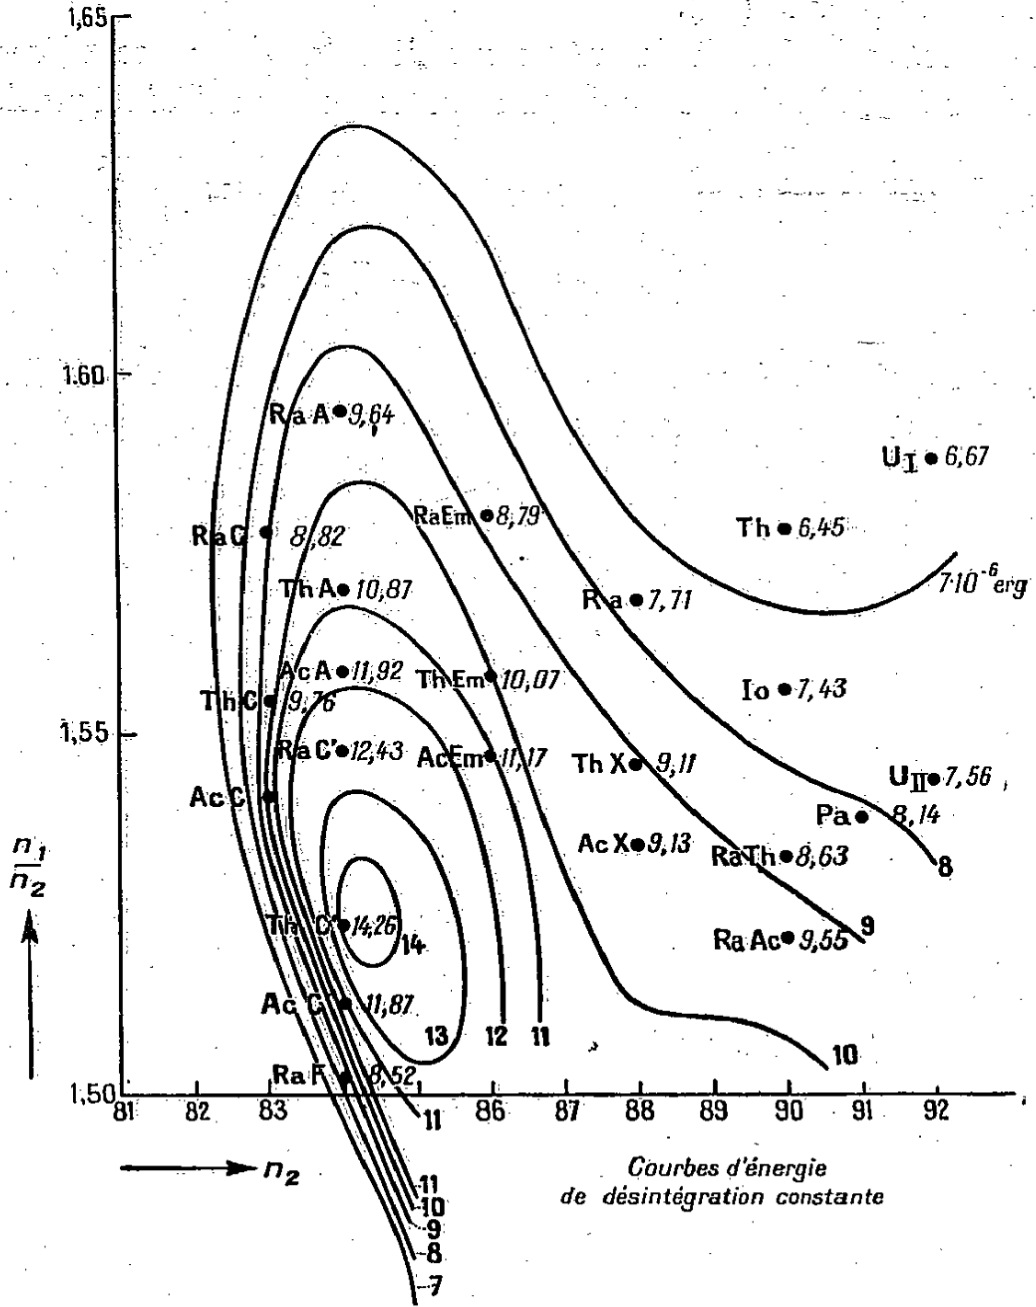
\includegraphics[width=300pt]{images/Fig10}
\end{figure}

Figure 9 clearly shows why there are no longer any stable nuclei beyond a certain nuclear charge determined by the intersection of two stability curves. However it must be recalled here that a method of calculating as approximate as Thomas-Fermi's may not take account of the particularities presented by the radioactive families. To make this fact clear, in figure 10 the curves of constant $\alpha$ decay energy are traced in the domain of these radioactive series, starting from the experimental data. One immediately verifies certain peculiarities (maximum decay energy for $\El{Th}\El{C}'$) which are not accounted for in a perfunctory theory of the structure of the nucleus. \?{The Thomas-Fermi method may only give the general appearance of the energy variation}{C'est seulement l'allure générale de la variation d'énergie que peut donner la méthode de Thomas-Fermi}.

So far we have used only a very small number of theoretical data for the mass defects of light nuclei. Wigner\footnote{\citeauthor{E. Wigner}, \citepub{Phys. Rev.}, \citevol{43}, \citeyear{1933}, \citepage{p. 252}.} has examined the extent to which the hypothesis of an ordinary action (not an exchange action) between the neutron and the proton may account for the fact that the mass defect of the isotope $\mnEl{1}{2}{H}$ is a fifth of that for the helium nucleus. He found that for a certain form of the action law, the energy of the $\mnEl{1}{2}{H}$ nucleus is notably weaker in absolute value than the mean potential energy or the mean kinetic energy of the particles in this nucleus. If that is so, the ratio of the mass defects of $\mnEl{4}{2}{He}$ and $\mnEl{1}{2}{H}$ is too large. Wigner's results may be extended immediately to Majorana's model.

\subsection{Scattering and decay.}

The hypotheses that nuclei are composed of neutrons and protons, and that there is a simple law of action between these two types of particles also permits simple applications to the theory of collisions between nuclei and $\alpha$ particles, protons and neutrons. In particular, one can easily deduce from the law of action between protons and neutrons that of the scattering of neutrons by protons; inversely, the experimental results concerning this scattering permits directly attaining the assumed-unknown law of action. Unfortunately the currently-available experimental material does not permit a precise determination of this law of action. As the theory of scattering and decay is treated in Gamow's report, only certain points concerning the neutron hypothesis in particular will be examined.

Iwanenko\footnote{\citeauthor{Iwanenko}, \textit{loc. cit}.} has interpreted the fact that the decay of beryllium nuclei under the action of $\alpha$ rays only emits neutrons and $\gamma$ rays without any proton in the following manner: the beryllium nucleus of mass 9 is composed, in the hypothesis used here, of two $\alpha$ particles and a neutron; as long as the energy of the incident $\alpha$ particle is not sufficient for the $\alpha$ particles themselves to decay, the nucleus omly emits neutrons. Pursuing the consequences of this idea, one likewise predicts an emission of neutrons in the bombardment of carbon by $\alpha$ particles ($\mnEl{6}{12}{C}$ may not decay, but the same considerations apply as for $\mnEl{4}{9}{Be}$ to the rare isotope $\mnEl{6}{14}{C}$); on the contrary one predicts a mix of neutrons and protons with $\El{Li}$, $\El{B}$, $\El{N}$ and $\El{O}$. If, like Cockroft and Walton\footnote{\citeauthor{Cockroft and Walton}, \citepub{Proc. Roy. Soc. A}, \citevol{137}, \citeyear{1932}, \citepage{p. 229}.}, we use protons to produce the decays, the emitted radiation may be composed of $\alpha$ particles and neutrons. It particular one can predict the appearance of neutrons with heavier nuclei ($\mnEl{17}{37}{Cl}$ for example) which contain several neutrons in addition to the $\alpha$ particles.

A particularly significant result of the Cockroft and Walton experiments\footnote{The recent research by Rutherford and Oliphant seems to show that Cockroft and Walton's results on the decay of very heavy elements are in reality due to secondary effects (\textit{cf.} Cockroft's report). The consoderations just alluded to by Teller nevertheless retain their importance for the discussion of the decay of lighter elements.} shows that the protons may likewise produce decay in heavy nuclei ($\El{Co}$, $\El{Pb}$, $\El{U}$), though with a very low yield. This result is incomprehensible if one considers the penetration of a proton into the nucleus as a necessary prior condition for decay. In fact, the probability that a proton with $500,000 \text{electron-volts}$ of energy can penetrate into a uranium nucleus is infinitely small. Teller\footnote{I am very indebted to M. Teller for an interesting discussion on these questions.} has remarked on this subject that the hypothesis of exchange action between neutrons and protons makes the process of an exchange in position between the incident proton and a neutron in the target nucleus possible. The neutron produced in this way consequently has the possibility of penetrating into the nucleus without having to cross Gamow's barrier due to the action of Coulomb forces. It follows that the diminution of the probability of decay as the atomic number increases is not in general represented by Gamow's exponential factor, and that the corresponding part of the exchange action diminishes approximately as $\left|J(r_\text{min})\right|^2$, where $r_\text{min}$ represents the distance to which the proton may approach the nucleus in the classical theory:
\uequ{
\frac{Ze^2}{r_\text{min}} = E_\text{kin}.
}
Then if $J(r)$ does not diminish too rapidly as the distance increases, the diminution of the probability may be much weaker than indicated by Gamow's factor. The experimental data corresponding to $J=a\exp{-br}$, $b=1.25\cdot 10^{12}\text{cm}^{-1}$, leading to a relatively slow diminution of $J$ when $r$ increases. However it remains uncertain if these considerations suffice for interpreting Cockroft and Walton's results for heavy nuclei.

\textsc{Note added in proof (1936-06-30).} — The discovery of radioactivity with emission of positrons (Joliot-Curie) demands modifying the preceding considerations a bit. In the rough approximation which is the basis of the equations (30) to (35), the only stable nuclei are in fact those for which $\left|\pXpY{E}{n_1} - \pXpY{E}{n_2}\right| \leq mc^2$. The stable nuclei are distributed symmetrically on both sides of the curve $\pXpY{E}{n_1} - \pXpY{E}{n_2}=0$. The width of the band of stable elements on either side of the curve will now however be given by the condition $\pXpY{E}{n_1} - \pXpY{E}{n_2} \leq mc^2$; on the contrary, the difference in energy between nuclei of even and odd charge has the effect of givinb this band, in the case of nuclei with even mass, a notably larger width than  the previous condition would predict. Details on this subject will be found in \textsc{W. Heisenberg}, \textit{loc. cit.}, II.



\end{document}